% file: jupiter-css-leftmost-transition.tex

\documentclass{standalone}

\usepackage{tikz}
\usetikzlibrary{shapes, positioning, arrows.meta, calc, backgrounds, fit}

% default horizontal/vertical distance
\def\hdist{1.5}
\def\vdist{1.5}

\newcommand{\state}[3]{% #1: state name; #2: position; #3: label
  \node (#1) [circle, inner sep = 0pt, minimum size = 10mm, text width = 10mm, align = center, draw, #2, font = \Large] {#3};
}

\newcommand{\trans}[3]{% #1: start state; #2: end state; #3: transition label position
  \draw[>=Stealth, ->, dashed] (#1) to node [rectangle, draw, above = 2pt, sloped, #3] {} (#2);
}

\newcommand{\transition}[4][]{% #2: start state; #3: end state; #4: transition label; #1: transition label position (optional)
  \draw[>=Stealth, ->] (#2) to node [rectangle, draw, above = 2pt, sloped, #1] {#4} (#3);
}

\begin{document}
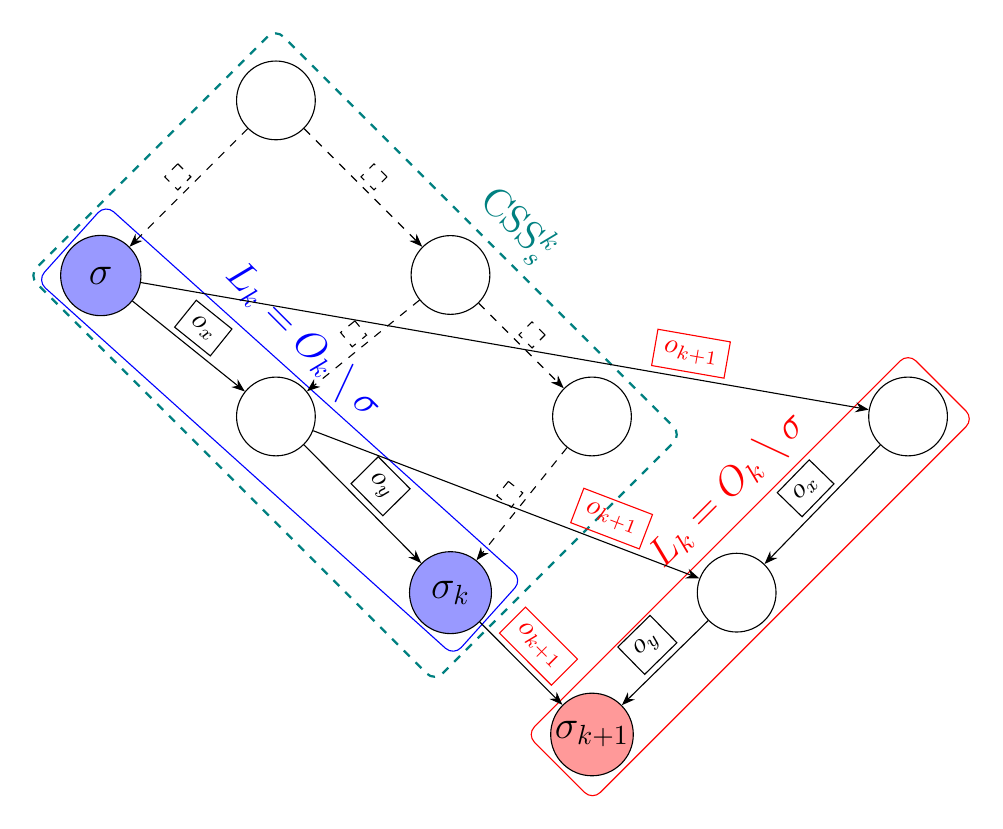
\begin{tikzpicture}[node distance = \vdist and \hdist,
  path/.style = {draw, rounded corners, very thick, #1}]
  \state{0}{}{}
  \state{1}{below left = of 0, fill = blue!40}{$\sigma$}
  \state{2}{below right = of 0}{}

  \state{12}{below = 2*\vdist of 0}{}
  \state{23}{right = 2*\hdist of 12}{}
  \state{14}{right = 2*\hdist of 23}{}
  
  \state{123}{below = 2*\vdist of 2, fill = blue!40}{$\sigma_k$}
  \state{124}{right = 2*\vdist - 0.40 of 123}{}

  \state{1234}{below = 2*\vdist of 23, fill = red!40}{$\sigma_{k+1}$}

  \trans{0}{1}{}
  \trans{0}{2}{}
  \transition{1}{12}{$o_x$}
  \trans{2}{12}{}

  \trans{2}{23}{}
  \trans{23}{123}{}
  \transition{12}{123}{$o_y$}

  \transition[near end, red]{1}{14}{$o_{k+1}$}
  \transition[near end, red]{12}{124}{$o_{k+1}$}
  \transition{14}{124}{$o_x$}

  \transition[red]{123}{1234}{$o_{k+1}$}
  \transition{124}{1234}{$o_y$}

  \begin{pgfonlayer}{background}
	\node (lk) [rectangle, draw = blue, rounded corners, rotate fit = 48, fit = (1) (12) (123), inner sep = 5pt, 
	  label = {[font = \Large, blue, rotate = -45] 40:$L_{k} = O_{k} \setminus \sigma$}] {};
  \end{pgfonlayer}

  \begin{pgfonlayer}{background}
	\node (lk) [rectangle, draw = red, rounded corners, rotate fit = 45, fit = (14) (124) (1234), inner sep = 6pt, 
	  label = {[font = \Large, red, rotate = 45] 46:$L_{k} = O_{k} \setminus \sigma$}] {};
  \end{pgfonlayer}

  \begin{pgfonlayer}{background}
	\node (lk) [rectangle, draw = teal, dashed, thick, rounded corners, rotate fit = 45, fit = (0) (1) (2) (12) (23) (123), inner sep = 8pt, 
	  label = {[font = \Large, teal, rotate = -45] 10:CSS$_{s}^{k}$}] {};
  \end{pgfonlayer}

  % \path [path = {red}] ($(0.center) + (135:5pt) + (45:20pt)$) node[above] {$C_1$} -- ($(1.center) + (135:5pt) + (225:5pt)$) 
  %   -- ($(1234.center) + (225:5pt)$);

  % \path [path = {blue}] ($(0.center) + (45:5pt) + (135:20pt)$) node[above] {$C_2$} -- ($(23.center) + (45:5pt) + (-45:5pt)$) 
  %   -- ($(123.center) + (-135:12pt) + (-45:5pt)$)
  %   -- ($(1234.center) + (-135:12pt)$);

  % \path [path = {teal}] ($(0.center) + (-45:5pt) + (45:20pt)$) node[above right] {$C_3$} -- ($(1.center) + (-45:5pt)$) 
  %   -- ($(14.center) + (-45:8pt)$)
  %   -- ($(1234.center) + (-45:8pt)$);
\end{tikzpicture}
\end{document}
